\documentclass[UEF8]{ctexart}
\usepackage{fontspec}
\setmainfont[Mapping=tex-text]{Noto Sans CJK TC Thin}
\usepackage[utf8]{inputenc}
\usepackage{indentfirst}
\usepackage{subcaption}
\usepackage{amsmath}
\usepackage{ctex}
\usepackage{amsfonts}
\usepackage{amssymb}
\usepackage{listings}
\usepackage{graphicx}
\usepackage{gensymb}
\usepackage{multicol}
\usepackage[a4paper,left=1cm,right=1cm,top=2cm,bottom=2cm]{geometry}
\usepackage{geometry}
%\setCJKmainfont[BoldFont=SimHei]{SimSun}
%\setCJKmonofont{SimSun}     
\parindent 2em 
\setlength{\columnseprule}{1pt}
\setlength\columnsep{1cm}

\title{直流非平衡电桥实验报告}
\author{余丰\quad PB19000261 \quad 705组}
\date{2020/12/8}


\begin{document}
\maketitle
{\bfseries 摘要} \quad 本次实验使用研究了桥臂电阻为$50,1K,5K\Omega$的等臂非平衡电桥的$U_{g}\sim\delta$关系以及其线性范围和灵敏度,后用桥臂电阻为50$\Omega$的等臂电桥测量了Cu丝的电阻和温度的关系。

\begin{multicols}{2}
\section{前言}
直流电桥是一种精密的电阻测量仪器,具有重要的应用价值。按电桥的测量
方式可分为平衡电桥和非平衡电桥。平衡电桥是把待测电阻与标准电阻进行比较,
通过调节电桥平衡,从而测得待测电阻值,如单臂直流电桥(惠斯登电桥)、双
臂直流电桥(开尔文电桥)。它们只能用于测量具有相对稳定状态的物理量,而
在实际工程和科学实验中,很多物理量是连续变化的,只能采用非平衡电桥才能
测量。

非平衡电桥的基本原理是通过桥式电路来测量电阻,根据电桥输出的不平衡
电压,再进行运算处理,从而得到引起电阻变化的其它物理量,如温度、压力、
形变等。
\section{实验方法}

\subsection{实验仪器}
稳压电源、电阻箱、万用表(用作毫伏表)、Keithy2000(用作微伏表)、铜
丝(漆包线)、加热台、温度计、导线等。
\subsection{实验原理}

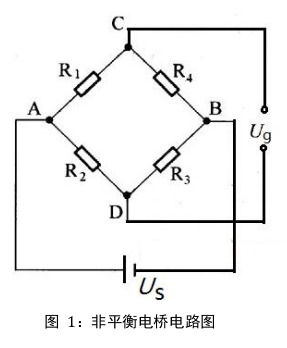
\includegraphics[scale=0.42]{graphs/p1.png}

 非平衡电桥原理如图 1 所示,当$\dfrac{R_{3}}{R_{2}}=\dfrac{R_{4}}{R_{1}}$时,电桥平衡,有$U_{g}=0$。当用$R_{4}+\Delta{R}$代替$R_{4}$时,$\dfrac{R_{3}}{R_{2}}$不等于$\dfrac{R_{4}+\Delta{R}}{R_{1}}$,此时$U_{g}$不等于 0,为非平衡状态。
 
 
$U_{g}$为数字电压表测量 C、D 二点输出电压(电压表内阻看着无穷大),应用
电路分析知识,可算出输出的非平衡电压为:
\begin{equation}
U_{g}=\dfrac{R_{2}R_{4}+R_{2}\Delta{R}-R_{1}R_{3}}{(R_{1}+R_{4})(R_{2}+R_{3})+\Delta{R}(R_{2}+R_{3})} \tag{1}
\end{equation}
分析上式,可以得到电桥的三种形式:
\begin{enumerate}
 	\item[(1)]等臂电桥:$R_{1}=R_{2}=R_{3}=R_{4}\equiv{R_{0}}$
 	\item[(2)]卧式电桥:$R_{1}=R_{4}$,$R_{2}=R_{3}$
 	\item[(3)]立式电桥:$R_{1}=R_{2}$,$R_{3}=R_{4}$
\end{enumerate}
将等臂条件代入(1)式经简化得:
\begin{equation}
U_{g}=\dfrac{U_{s}}{4}\delta\dfrac{1}{1+\dfrac{1}{2}\delta} \tag{2}
\end{equation}
其中$\delta=\dfrac{\Delta{R}}{R_{0}}$称为电阻的应变量,或叫“相对改变量”。我们在设计电桥时,令$\Delta{R}\ll{R_{0}}$,则$\delta\to{0}$,于是有:
\begin{equation}
U_{g}=\dfrac{U_{s}}{4}\delta=\dfrac{U_{s}}{4R_{0}}\Delta{R} \tag{3}
\end{equation}
 
 这样,非平衡电桥输出电压$U_{g}$与桥臂电阻的变化量$\Delta{R}$成正比,为线性关系。当$\Delta{R}$大时,(2)式中的$\dfrac{\delta}{2}$项不能省略,此时$U_{g}=\dfrac{U_{s}}{4}\delta\dfrac{1}{1+\dfrac{1}{2}\delta}$呈非线性关系。


\subsection{实验步骤}
\subsubsection{等臂非平衡电桥灵敏度和线性范围测量}
\begin{enumerate}	
	\item[1)] 调节电源输出电压,同时用万用表直流电压档来校准,使输出电压为
	$U_{s}=2.0V$。电路如图1所示并用导线连接好,用台式万用表(Keithy2000)来测量$U_{g}$。
	\item[2)]
	先取电桥为等臂,即:$R_{1}=R_{2}=R_{3}=R_{4}\equiv{R_{0}}=1K\Omega$由于导线有一定的电阻,微调改变$R_{3}$的值,使$U_{g}$为零,此时电桥平衡。
	\item[3)]改变$R_{4}$从$800\sim1200\Omega$,每次变化量为$20\Omega$,按顺序记下各$U_{g}$的值,将数据填入表1中,作出$U_{g}\sim\delta$(或$U_{g}\sim\Delta{R}$)曲线
	\item[4)]将$R_{0}$改为$50、5K\Omega$,重复上面三个步骤,测得$50、5K\Omega$的$U_{g}\sim\delta$(或$U_{g}\sim\Delta{R}$)曲线。
\end{enumerate}

\subsubsection{使用非平衡电桥测Cu丝电阻与温度关系}
\begin{enumerate}	
	\item[1)] 取桥臂电阻为$50\Omega$,用 Keithy2000(精度可以到1μV,使
	用最小量程100mV)来测量桥路输出电压$U_{g}$。保持恒压源输出电压为2.0V,微调$R_{3}$使电桥平衡(即:使$U_{g}$尽可能地小,越小越好。一般情况下,接近于或小于0.01mV)。平衡后,记录对应的$U_{g0}$。
	\item[2)] 把3m长,直径为0.60mm的Cu丝(漆包线,电阻率$\rho=1.687\times 10^{-8}\Omega/m$)
	串联到$R_{4}$所在的桥臂上。把Cu丝浸没到杯内水中,用温度计测量水温t,记录水温并测量当前水温下桥路输出电压$U_{g}$值。并与没有串联Cu丝时$U_{g0}$比较,计算Cu丝的当前温度下的电阻值$R_{Cu}$。
	\item[3)]用加热台对杯子进行加热,铜丝温度缓慢上升。每隔5°C记录一下对
	应的$U_{g}$值,直到85°C为止。
\end{enumerate}

\section{实验现象及数据处理}
\subsection{电阻为$50,1K,50K\Omega$的等臂非平衡电桥的灵敏度和线性范围}
数据使用mathematica处理,$U_{g}$与$R$的图像使用3次内插拟合得到,代码如下
\begin{lstlisting}[language=Mathematica]
dataf = Interpolation[datapoints
, InterpolationOrder -> 3, 
Method -> "Spline"];
\end{lstlisting}

求解相对误差等于0.05的方程即可得到线性范围的上下解
\begin{lstlisting}[language=Mathematica]
(R /. FindRoot[
Abs[(dataf[R] - dataintheoryf[R])
/dataintheoryf[R]] == 0.05, 
{R, {R0 + (1 - (ndata + 1)/2)
*steplength*R0, R0 + (ndata - 
(ndata + 1)/2)*steplength*R0}}])/R0
\end{lstlisting}

\subsubsection{$50\Omega$的等臂非平衡电桥的灵敏度和线性范围}
$U_{g}\sim{R_{4}}$图像:

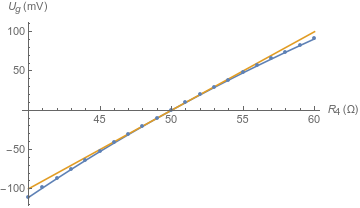
\includegraphics[scale=0.6]{graphs/data50.png}

相对误差$\delta{U_{g}}$与$R_{4}$图像:

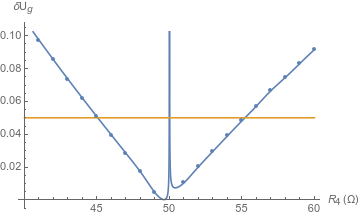
\includegraphics[scale=0.6]{graphs/data50error.png}

通过计算得线性范围为$R_{4}$:$45.0543\sim55.2051\Omega$,$\delta:-0.0989142\sim0.104102$,$\Delta{R}=\dfrac{R_{4R}-R{4L}}{2}=\dfrac{55.2051\Omega-45.0543\Omega}{2}=5.0754\Omega$,$\delta$的范围$\delta{R}=\Delta{R}/R0=0.101508$。灵敏度由(3)式可得$S_{Uabs}=10mV/\Omega$。

\subsubsection{$1K\Omega$的等臂非平衡电桥的灵敏度和线性范围}
$U_{g}\sim{R_{4}}$图像:

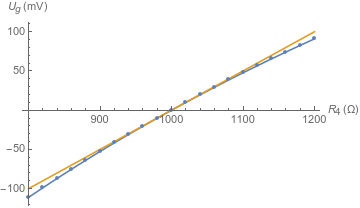
\includegraphics[scale=0.6]{graphs/data1K.png}

相对误差$\delta{U_{g}}$与$R_{4}$图像:

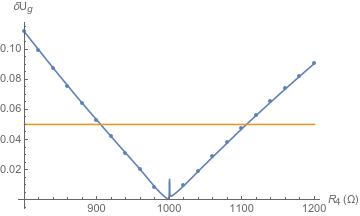
\includegraphics[scale=0.6]{graphs/data1Kerror.png}

通过计算得线性范围为$R_{4}$:$905.018\sim1106.22\Omega$,$\delta:-0.0949818\sim0.106217$,$\Delta{R}=\dfrac{R_{4R}-R{4L}}{2}=\dfrac{1106.22\Omega-905.018\Omega}{2}=100.601\Omega$,$\delta{R}=\Delta{R}/R0=0.100601$。灵敏度由(3)式可得$S_{Uabs}=0.5mV/\Omega$。

\subsubsection{$5K\Omega$的等臂非平衡电桥的灵敏度和线性范围}
$U_{g}\sim{R_{4}}$图像:

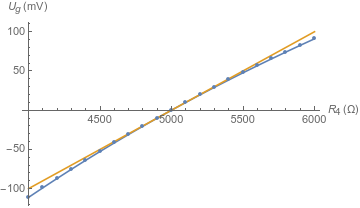
\includegraphics[scale=0.6]{graphs/data5K.png}

相对误差$\delta{U_{g}}$与$R_{4}$图像:

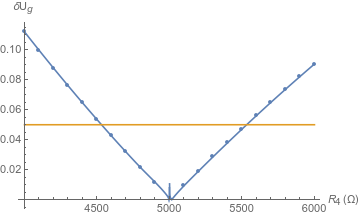
\includegraphics[scale=0.6]{graphs/data5Kerror.png}

通过计算得线性范围为$R_{4}$:$4531.26\sim5532.43\Omega$,$\delta:-0.0937475\sim0.106486$,$\Delta{R}=\dfrac{R_{4R}-R{4L}}{2}=\dfrac{5532.43\Omega-4531.26\Omega}{2}=500.585\Omega$,$\delta{R}=\Delta{R}/R0=0.100117$。灵敏度由(3)式可得$S_{Uabs}=0.1mV/\Omega$。



由此可见,$\delta$的线性范围几乎不随的等臂非平衡电桥电阻$R_{0}$改变,而但电源电压恒定时,$R_{0}$越小,非平衡电桥的灵敏度$S_{abs}$越大。
\subsection{铜丝电阻温度系数以及其不确定度计算}
\subsubsection{铜丝电阻温度系数的计算}
C、D电压差$U_{g}$与温度$T$线性拟合图像:
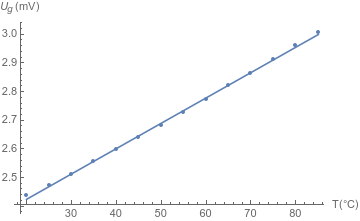
\includegraphics[scale=0.55]{graphs/OriginaldataCU.png}

使用mathematica的LinearModelFit得到(ConfidenceLevel -> 0.95)

\small
$$\begin{array}{l|lll}
	\text{} & \text{Estimate} & \text{Standard Error} & \text{Confidence Interval} \\
	\hline
	1 & 2.24689 & 0.00474749 & \{2.23655,2.25724\} \\
	\text{T} & 0.00884813 & 0.0000844207 & \{0.0086642,0.00903207\} \\
\end{array}$$
相关系数RSquared=$\rho_{b,m}=\rho_{m,b}=0.998909$

\normalsize
从上表中读出截距$b=2.24689mV$,斜率$m=0.00884813mV/(^\circ{C})$。
上面$50\Omega$电阻非平衡电桥的灵敏度为$S_{Uabs}=10mV/\Omega$。

$0^\circ{C}$时Cu丝电阻$R_{0^\circ{C}}=b/S_{Uabs}=0.224689\Omega$。$0^\circ{C}$处铜丝温度系数为$\aleph_{0^\circ{C}}=\dfrac{m}{b}=3.757\times10^{-3}(^\circ{C})^{-1}$。

$20^\circ{C}$时Cu丝电阻$R_{20^\circ{C}}=(b+m*20)/S_{Uabs}=0.240165\Omega$。$20^\circ{C}$处铜丝温度系数为$\aleph_{0^\circ{C}}=\dfrac{m}{b+m*20}=3.684\times10^{-3}(^\circ{C})^{-1}$。

\subsection{Cu丝在$0^\circ{C}$和$20^\circ{C}$时电阻温度系数$\alpha_{0^\circ{C}}$和$\alpha_{20^\circ{C}}$的不确定度计算}
由上面表格知:
\begin{equation*}
\begin{aligned}
& b=2.24689mV\\
& m=0.00884813mV/(^\circ{C}) \\
& \sigma_{b}=0.00474749mV \\
& \sigma_{m}=0.0000844207mV/(^\circ{C}) \\
& \rho_{b,m}=\rho_{m,b}=0.998909
\end{aligned}
\end{equation*}

\subsubsection{$0^\circ{C}$时电阻温度系数不确定度计算}
	当n=14,p=0.95时,tp=2.179。
\begin{equation*}
\begin{aligned}
U_{ma}&=tp\sigma_{m} \\
& = 2.179\times{0.0000844207mV/\Omega} \\
& =1.83953\times10^{-4}mV/(^\circ{C})\\
U_{ba}&=tp\sigma_{b} \\
& = 2.179\times{0.00474749mV} \\
& =1.03448\times10^{-2}mV \\
m&=8.66418\times10^{-3}mV/(^\circ{C})\sim9.03208\times10^{-3}mV/(^\circ{C}) \\
b&=2.23655\Omega\sim2.25723\Omega 
\end{aligned}
\end{equation*}
这与上表中给出的m的范围$\{0.0086642,0.00903207\}$,b的范围$\{2.23655,2.25724\}$基本一样。

\begin{equation*}
\begin{aligned}
\dfrac{U_{\alpha_{0}}}{\alpha_{0}}&=\sqrt{(\dfrac{U_{ba}}{b})^2+(\dfrac{U_{ma}}{m})^2-2\rho_{b,m}(\dfrac{U_{ba}}{b})(\dfrac{U_{ma}}{m})} \\
&=0.0161924 \\
U_{\alpha_{0^\circ{C}}}&=\alpha_{0^\circ{C}}\times 0.0161924 \\
&=6.08346\times 10^{-5}(^\circ{C})^{-1}
\end{aligned}
\end{equation*}
故$0^\circ{C}$处的电阻温度系数为:
\begin{equation*}
\begin{aligned}
\alpha_{0^\circ{C}}=(3.76\pm 0.06)\times 10^{-3}(^\circ{C})^{-1}
\end{aligned}
\end{equation*}

\subsubsection{$20^\circ{C}$时电阻温度系数不确定度计算}
当n=14,p=0.95时,tp=2.179。在线性拟合时将横坐标减去20可得$20^\circ{C}$时的截距和方差。
\small
$$
\begin{array}{l|lll}
	\text{} & \text{Estimate} & \text{Standard Error} & \text{Confidence Interval} \\
	\hline
	1 & 2.42386 & 0.00322847 & \{2.41682,2.43089\} \\
	\text{T} & 0.00884813 & 0.0000844207 & \{0.0086642,0.00903207\} \\
\end{array}
$$
相关系数RSquared=$\rho_{b,m}=\rho_{m,b}=0.998909$
\normalsize

\begin{equation*}
\begin{aligned}
U_{ma}&=tp\sigma_{m} \\
& = 2.179\times{0.0000844207mV/\Omega} \\
& =1.83953\times10^{-4}mV/(^\circ{C})\\
U_{ba}&=tp\sigma_{b} \\
& = 2.179\times{0.00322847mV} \\
& =7.03484\times10^{-3}mV \\
m&=8.66418\times10^{-3}mV/(^\circ{C})\sim9.03208\times10^{-3}mV/(^\circ{C}) \\
b&=2.416825\Omega\sim2.43089\Omega 
\end{aligned}
\end{equation*}

\begin{equation*}
\begin{aligned}
\dfrac{U_{\alpha_{0}}}{\alpha_{0}}&=\sqrt{(\dfrac{U_{ba}}{b})^2+(\dfrac{U_{ma}}{m})^2-2\rho_{b,m}(\dfrac{U_{ba}}{b})(\dfrac{U_{ma}}{m})} \\
&=0.0178914 \\
U_{\alpha_{20^\circ{C}}}&=\alpha_{20^\circ{C}}\times 0.0178914 \\
&=6.59119\times 10^{-5}(^\circ{C})^{-1}
\end{aligned}
\end{equation*}
故$20^\circ{C}$处的电阻温度系数为:
\begin{equation*}
\begin{aligned}
\alpha_{0}=(3.68\pm 0.07)\times 10^{-3}(^\circ{C})^{-1}
\end{aligned}
\end{equation*}
\subsection{结果分析}
温度为$0^\circ{C}$时的电阻温度系数参考值为$0.00393(^\circ{C})^{-1}$,测量值$(3.76\pm 0.06)\times 10^{-3}(^\circ{C})^{-1}$相较其明显偏小且参考值并没有落在测量值的范围之内,说明有较大系统误差,下面列举一些可能导致测量值偏差的因素:

\begin{enumerate}
	\item[(1)]水升温太快导致铜丝温度始终低于水,铜丝温度变化相较与水的偏小,导致实测的$\Delta{T}$偏大,使计算出的电阻温度系数偏小。
	\item[(2)]非平衡电桥线性范围内仍有实测电压低于理论电压的情况,导致实际倒推回的测量的电阻阻值相较实际偏小,导致电阻温度系数偏小
\end{enumerate}

\subsection{实验思考题}
1. 简述直流非平衡电桥与直流平衡电桥的关系。\\
答:直流平衡电桥采用电桥平衡时的电阻比值的关系来测量待测电阻,而直流非平衡电桥则是通过计算有一桥电阻改变时的动态关系来测量待测电阻,直流非平衡电桥相较于直流平衡电桥测量误差较大但便于测量容易变化的电阻。

2. 为什么在实验内容1中,$R_{4}$的绝对值相同时,$R_{4}$小于1000Ω时的$U_{g}$值
比$R_{4}$大于1000Ω时的$U_{g}$值,绝对值大? \\
答:$R_{4}$较偏离平衡点时$U_{g}=\dfrac{U_{s}}{4}\dfrac{\delta}{1+\dfrac{1}{2}\delta}$,当$\delta$小于0时,分母小于1,分子的绝对值又与$-\delta$的绝对值相同,故整体的绝对值大于$\delta$大于0时的情况。故$U_{g}$的偏差的绝对值在$R_{4}$小于$1K\Omega$时的大于在$R_{4}$大于$1K\Omega$时的。

3. 假设用非平衡电桥来测量一个热敏电阻的电阻值随温度的变化,$U_{s}=2.0V$,毫伏表最小刻度为1mV,在室温(35°C)到85°C度范围内,热敏电阻的电阻值改变50Ω,取等臂电桥,为了保证测量的灵敏度(即:每隔 5°C读一次输出电压值,变化量不小于1mV)并且保持(与理论线性之间的误差小于)5\%的线性范围,请问$R_{0}$取多少比较合适?(指取值范围的上下限。) \\
答:平均下来每$5^\circ{C}$的变化的电阻阻值为$\Delta{R}=5\Omega$,而电压变化量不小于1mV,这说明$S_{abs}=\dfrac{U_{s}}{4R_{0}}>=0.2mV/\Omega$,即$R_{0}<=2500\Omega$。由$1K\Omega$的测量数据知$\dfrac{50\Omega}{R_{0}}=\delta{R}<=0.100601$,$R_{0}>=\dfrac{50\Omega}{0.100601}=497.013\Omega$。所以$R_{4}=497.013\sim 2500\Omega$

4. 把计算出来的Cu丝电阻温度系数与参考值$0.00393(^\circ{C})^{-1}$进行比较并分析。 \\
答:参考前面结果分析部分。

\section{结论}
本次实验测量了电阻分别为$50,1K,50K\Omega$的等臂非平衡电桥的灵敏度和线性范围,,并使用直流非平衡电桥间接测量了Cu丝电阻温度系数,证明非平衡电桥根据电桥输出的不平衡电压,再进行运算处理,可以测量引起电阻变化的其它物理量,如温度、压力、形变等。

\section{参考文献}
\begin{enumerate}
	\item[[1]] 大学物理实验(第二册第二版),谢行怒、康士秀、霍剑青,高等教育出版社,2005.11,ISBN 7-04-017774-9
	\item[[2]] 直流非平衡电桥实验讲义,黄双安,中国科学技术大学,2020.11.19 
\end{enumerate}
\small
注:本实验报告相关内容(如数据处理程序以及latex文档源代码)可以访问下面网址得到:\\
https://github.com/hubaak/data-processing-program-of-college-physices-experiment-for-ustcer


\end{multicols}
\end{document}
